\outline{1}{Learning, Not Recovery, is Modulated by Joint Synergies and Redundancy Exploration in Robotic Training Post-Stroke}
\chapter{Learning, Not Recovery, is Modulated by Joint Synergies and Redundancy Exploration in Robotic Training Post-Stroke}
\label{cha:armeospring}



\outline{2}{Introduction}
\section{Introduction}



\outline{2}{Methods}
\section{Methods}

\subsection{Data Collection}

\textbf{Participants.} 
We recruited 11 young (age 23 $\pm$ 2) healthy subjects (7 males) as the control group.
We recruited 53 post-stroke individuals with gender and affected side balanced, shown in table \ref{tab:demog}. 
Participants receive conventional rehabilitation besides robot-aided rehabilitation.

\begin{table}[b]
	\begin{tabular}{c c c c c c c c}
		\hline
		Group & No. & Age & Affected Side & Gender & FM(0-66) & Post Stroke Days & No. of Tests\\
		\hline
		Stroke & 53 & 59$\pm$14 & 29L, 24R & 19F, 30M & 25$\pm$9 to 39$\pm$ 14 & 56$\pm$21 & 80 in 4 weeks \\ 
		Control & 11 & 23$\pm$2 & - & 4F, 7M & - & - & 20 in 1 weeks \\
		\hline
	\end{tabular}
	\caption{Participants information}
	\label{tab:demog}
\end{table}

\textbf{Device.}
Our robot-aided rehabilitation uses ArmeoSpring exoskeleton \cite{} for therapy training. 
Shown in figure \ref{fig:1setupschedule}, the exoskeleton has 6 degrees of freedom, summarized in table \ref{tab:devicedof} and Fig. \ref{fig:1setupschedule}B. 
It is attached to the arm by two or three velcro straps. 
The exoskeleton has two springs equipped, at the upper arm and the forearm respectively. 
The springs can be adjusted to compensate the gravity force of the arm. 
Lengths of the exoskeleton are also adjustable to adapt to user's arm length.
There are no motors at any joints, user has to move actively to control the exoskeleton. 
User's trunk is mildly constrained by the velcro strap at the upper arm.


\begin{table}
	\begin{tabular}{c c c c}
		\hline
		Joint No. & Joint Name & Anatomical Counterpart & Direction \\
		\hline
		1(a) & Inner Shoulder Angle & Shoulder Horizontal Ab-/Adduction & Left/Right \\
		1(b) & Outer Shoulder Angle & Shoulder Horizontal Ab-/Adduction & Left/Right \\
		2 & Upper Arm Angle & Shoulder Flex-/Extension & Up/Down \\
		3 & Elbow Angle & - & Left/Right \\
		4 & Forearm Angle & - & Up/Down \\
		5 & Pro-/Supination Angle & Pro-/Supination & - \\ 
		6 & Flex-/Extension Angle & Wrist Flex-/Extension & - \\
		\hline
	\end{tabular}
	\caption{Degrees of freedom of ArmeoSpring exoskeleton.}
	\label{tab:devicedof}
\end{table}

The device records all joint angles (that is, the joints of the exoskeleton), and calculates the end effector location through a forward kinematics model of the exoskeleton. 
The end effector location then is used to control a cursor on a screen, displayed vertically in front of the user. 
All joint angles and end effector locations are recorded.

\textbf{Training and Test.}
Participants in the control group receive two training sessions (morning and afternoon) for five consecutive days in a week.
Post-stroke participants receive the same amount of training per day every weekday for 4 consecutive weeks (Fig. \ref{fig:1setupschedule}C).

One training session consists of several games, each lasts at most 3 minutes (with the exception of the ladybug pointing test mentioned below).
One training session typically lasts about 20 minutes.

A ladybug pointing test is scheduled at the beginning and the end of each training session. 
This test is two-dimensional; the movement along the dimension perpendicular to the screen is ignored. 
In this test, the user tries to catch ladybugs that appear one by one pseudo randomly on the screen. 
The sequence of locations that ladybugs appear are fixed, although within a test they seem random.
To catch the ladybug, the user moves the cursor to its location. 
The user has limited time to catch the ladybug.
After a ladybug is caught, or the time limit is reached, the ladybug disappears and the next ladybug appears somewhere else. 

\subsection{Data Analysis}

\textbf{Preprocessing.}
We filter the data with a second order Butterworth filter with a cutoff frequency of 5 Hz.
We define a trial as the movement between two consecutive ladybugs.
A trial is considered successful if it starts from previously caught target and leads to the catching of next target. 
Only successful trials (control 99.8\%, stroke 78.2\%) are included in task space performance analysis.
We also exclude tests in which participants caught less than 25\% ladybugs (that is 0.7\% of all tests).

\textbf{Task Space Performance.}
We characterize task space performance of a ladybug test via the average number of peaks in the velocity profile \cite{}. 
To calculate the number of peaks in a velocity profile of a trial, we take the derivative of velocity (tangential acceleration) and count the number of times it goes from positive to negative.
We then take the average of number of peaks ($ p $) of all successful trials in the test.

We model the dynamics of number of peaks $ p $ as exponential functions of time $ t $ represented by task number.
For participants in the control group, we consider a single exponential function
\begin{equation}\label{eqn:singleexp}
p = a e^{-b t} + 1
\end{equation}
where $ t $ is test number, $ b $ is learning rate.
We choose an asymptote of 1 because it is the theoretical limit of number of peaks.

For participants in the stroke group, we consider two exponential components to model the number of peaks
\begin{equation}\label{eqn:doubleexp}
p = a_1 e^{-b_1 t} + a_2 e^{-b_2 t} + 1
\end{equation}
$ a_1, a_2, b_1 $ and $ b_2 $ are constraint to be positive.
For convenience, we assume $ b_1 > b_2 $.

We fit nonlinear mixed effect models \cite{} to equation \ref{eqn:singleexp} and \ref{eqn:doubleexp} via Matlab 2016a function \textsf{nlmefit}.
The results of mixed effect model include the fixed effect $ \hat{a} $ and $ \hat{b} $ that represents group average, and the random effect for each participant $ a_s $ and $ b_s, s = 1, ..., N_\text{sb} $.

\textbf{Joint Space Variability.}
Because the last two joints (pronation/supination and wrist angle) have relatively small variance (control 12.4\%, stroke 4.6\%), we ignore them during joint space variability analysis and synergy analysis.
To quantify joint space variability and its relevance to the task space, we use a nonlinear forward kinematics model of the exoskeleton (cite company \cite{})
	\begin{equation}\label{eqn:nonlinearForwardKinematics}
	\bm{r} = f(\bm{\theta})
	\end{equation}
where $ \bm{r} = (x,y)^T $ is the location of the end effector, $ \bm{\theta} $ is joint angles (see Table \ref{tab:devicedof} and Fig. \ref{fig:1setupschedule}B for details). 
The distribution of variability for each target(ladybug) is calculated from the last 10 tests at the moment of catching the ladybug. 

The mean joint configuration across the last 10 tests at one specific ladybug ($ b $) is denoted by $ \bar{\bm{\theta}}_b $.
We will omit index $ b $ for convenience.
The Jacobian matrix at configuration $ \bar{\bm{\theta}} $ is obtained through forward kinematics (Eqn. \ref{eqn:nonlinearForwardKinematics})
	\begin{equation}
	\bm{J}(\bar{\bm{\theta}}) = \frac{\partial f(\bm{\theta})}{\partial \bm{\theta}} \Big\rvert_{\bar{\bm{\theta}}}
	\end{equation}
which is a 2 by 4 matrix.
The null space of Jacobian $ \bm{J} $ can be represented by basis of the space $ \bm{\xi}_i $, $ i= 1,2 $ which satisfy
	\begin{equation}
	\bm{J}(\bar{\bm{\theta}}) \bm{\xi}_i = 0
	\end{equation}
This means that movements in the null space ($ \bm{\xi}_i $) have no effect on the location of end effector, hence is task irrelevant.
Therefore we also call the null space as the task-irrelevant space.
For a specific test ($ t $) , the deviation of joint angles from $ \bar{\bm{\theta}} $ is
	\begin{equation}
	\Delta\bm{\theta}_t = \bm{\theta}_t - \bar{\bm{\theta}}
	\end{equation}
We will omit index $ t $ as well.
The projection of $ \Delta\bm{\theta} $ to the task-irrelevant space is
	\begin{equation}
	\Delta\bm{\theta}_{\text{null}} = \sum_i^m \langle \Delta\bm{\theta}, \bm{\xi}_i \rangle \bm{\xi}_i, m=2
	\end{equation}
where $ \langle,\rangle $ represents inner product.
In the end, we quantify the task-irrelevant variability by calculating the mean of squared $ \Delta\bm{\theta}_{\text{null}} $
	\begin{equation}\label{eqn:nullvar}
	V_{\text{null}}(t,b) = \mathbb{E}_{t,b} (\Delta\bm{\theta}_{\text{null}}^T\Delta\bm{\theta}_{\text{null}})
	\end{equation}
where $ t,b $ index tests and targets (ladybugs). 
We then average $ V_{\text{null}}(t,b) $ across tests ($ t $) and targets ($ b $) as the measure of task-irrelevant variability of a participant. 
Because $ V_{\text{null}} $ is similar to the calculation of variance, it has unit of $ \text{deg}^2 $.
It is on average the summation of variance across all joints.

To obtain variability in the orthogonal (task-relevant) space, we simply replace $ \bm{\xi}_i $ with the basis of the orthogonal space, $ \bm{\psi}_i $, $ i= 1,2 $  :
	\begin{equation}
	\Delta\bm{\theta}_{\text{orth}} = \sum_i^m \langle \Delta\bm{\theta}, \bm{\psi}_i \rangle \bm{\psi}_i, m=2
	\end{equation}
and the task-relevant space variability is
	\begin{equation}\label{eqn:taskvar}
	V_{\text{orth}}(t,b) = \mathbb{E}_{t,b} (\Delta\bm{\theta}_{\text{orth}}^T\Delta\bm{\theta}_{\text{orth}})
	\end{equation}

\textbf{Synergy Extraction and Analysis.}
We use Principal Component Analysis (PCA) to extract joint synergies from each ladybug test.
PCA belongs to a family of Dimension Reduction methods.
Principal Components of joint angles, which captures most of the variance presented in the data, can be interpreted as joint synergies \cite{}.
In this study, we only look at the first two synergies which on average account for 83.9\% joint angle variance for control group, 83.1\% for stroke group.
Joint synergies of healthy participants are quite stable across individuals.
We calculate the averaged synergies shown in figure \ref{fig:6synergy}C.

To evaluate the synergy pattern of stroke participant, we use the principal angle \cite{} between subspaces that are spanned by synergies \cite{}.
Generally, the principal angle $ \phi $ between two subspaces is the minimum rotation angle required to rotate one subspace onto the other.
A principal angle of \ang{0} indicates the same synergy patterns, whereas \ang{90} indicates completely different ones.
Therefore we refer to this angle as synergy abnormality.
We use Matlab 2016a \textsf{subspace} \cite{} to calculate the principal angle. 

For each stroke participant, we investigate the synergy abnormality (principal angle) $ \phi $ between his synergies from every test and the average healthy synergies.
$ \phi(t) $ ($ t $ for test) reflects the abnormality of participant's joint synergy patterns throughout training. 
We fit a linear mixed effect model to $ \phi(t) $ with a fixed effect on the intercept $ \phi(0) $ and a random effect on both the intercept and slope (we do not include a fixed effect on the slope because it is not significant when included in the model).
%The intercept $ \phi(0) $ tells us how different this participant's synergy pattern is initially different from the control group.
%It is therefore a measure of joint coordination prior training.

To investigate how joint synergies affects task space learning, we correlate $ \phi(0) $ with task space (fast and slow) learning rate.

\textbf{Linear Regression}
In this study, when doing linear regression, we identify outliers through Cook's Distance \cite{}.
Instead of removing them, we adopt robust regression method with the bisquare weight function \cite{}.

\outline{2}{Results}
\section{Results}

Stroke participants show significant changes after training in kinematics performance.
Fig. \ref{fig:2stroketrajexamp} shows representative trajectories in both task space and joint space. 
After training, the trajectories in task space are straighter, and the joint trajectories also seem smoother. 
%In this particular trial in Fig. \ref{fig:2stroketrajexamp}B, the movement time is also shorter.

\textbf{Task Space Performance.}
Fig. \ref{fig:3nopfixran} shows the number of peaks modeled by exponential functions.
Control subjects show much fewer number of peaks on average (Fig. \ref{fig:3nopfixran}A).
Stroke participants show significant improvement (Fig. \ref{fig:3nopfixran}B), although still more than control group at the end of training.

The double exponential mixed effect model (Eqn. \ref{eqn:doubleexp}) gives two learning rates $ b_1 $ and $ b_2 $. 
We refer the smaller of the two, $ b_2 $ as the slow learning rate, the bigger, $ b_1 $ the fast learning rate.
Fig. \ref{fig:3nopfixran}C shows examples of individual fitting.
The slow component, due to small learning rate, is essentially linear; but the fast component usually goes to asymptote during the training.

To interpret these two fitted learning rates, we compare them with Fugul Meyer (FM) assessment score \cite{}.
The post training number of peaks and post training FM are significantly correlated ($ p = 0.0003 $, Fig. \ref{fig:4slowcomponentisrecovery}A).
This indicates that the number of peaks is a good measurement of abnormal synergy patterns.
In addition, the change of number of peaks before and after training due to the slow process (term $ a_2e^{-b_2t} $ in Eqn. \ref{eqn:doubleexp}), correlates significantly ($ p<0.0001 $) with the change of FM (Fig. \ref{fig:4slowcomponentisrecovery}B).
This further indicates that the slow learning process, rather than the fast one, reflects a recovery of synergy patterns.
We therefore refer to $ b_2 $ as the recovery rate, and $ b_1 $ as the learning rate.

\textbf{Joint Space Variability.}
Both control group and stroke group display much larger task-irrelevant variability than task-relevant variability.
For example, for the control group, the task-irrelevant variability on average is $ \ang{18.3} \pm \ang{19.4} $ (measured by standard deviation, $ \sqrt{V_\text{null}} $); whereas the task-relevant variability ($ \sqrt{V_\text{orth}} $) on average is $ \ang{3.1} \pm \ang{2.9} $.

Task-irrelevant variability positively correlates with the learning rate $ b_1 $ (see Eqn. \ref{eqn:doubleexp}), as shown in Fig. \ref{fig:5learnratevsnullvar}.
Participants with small task-irrelevant variability learn slower (such as SB 46, see Fig. \ref{fig:3nopfixran}C: SB 46);
participants with large tasl-irrelevant variability learn faster (such as SB 46, see Fig. \ref{fig:3nopfixran}C: SB 53);

\textbf{Synergy Analysis.}
We identify two synergies from control group, as shown in Fig. \ref{fig:6synergy}C.
The first synergy is composed of Shoulder Horizontal (SH) rotation and Elbow (EL) angle, and it is responsible for horizontal movements.
The second synergy is composed of Shoulder Elevation (SE) angle and Forearm (FA) angle, and it is responsible for vertical movements.

We are not able to identify stable synergies from stroke participants due to large differences across different participants.
They can share a similar structure as the control group (Fig. \ref{fig:6synergy}B), or have different structure (Fig. \ref{fig:6synergy}A).

The initial synergy abnormality correlates with the recovery rate $ b_2 $ (see Eqn. \ref{eqn:doubleexp}) as shown in Fig. \ref{fig:6synergy}D.


\outline{2}{Discussion}
\section{Discussion}



\begin{figure}
	\centering
	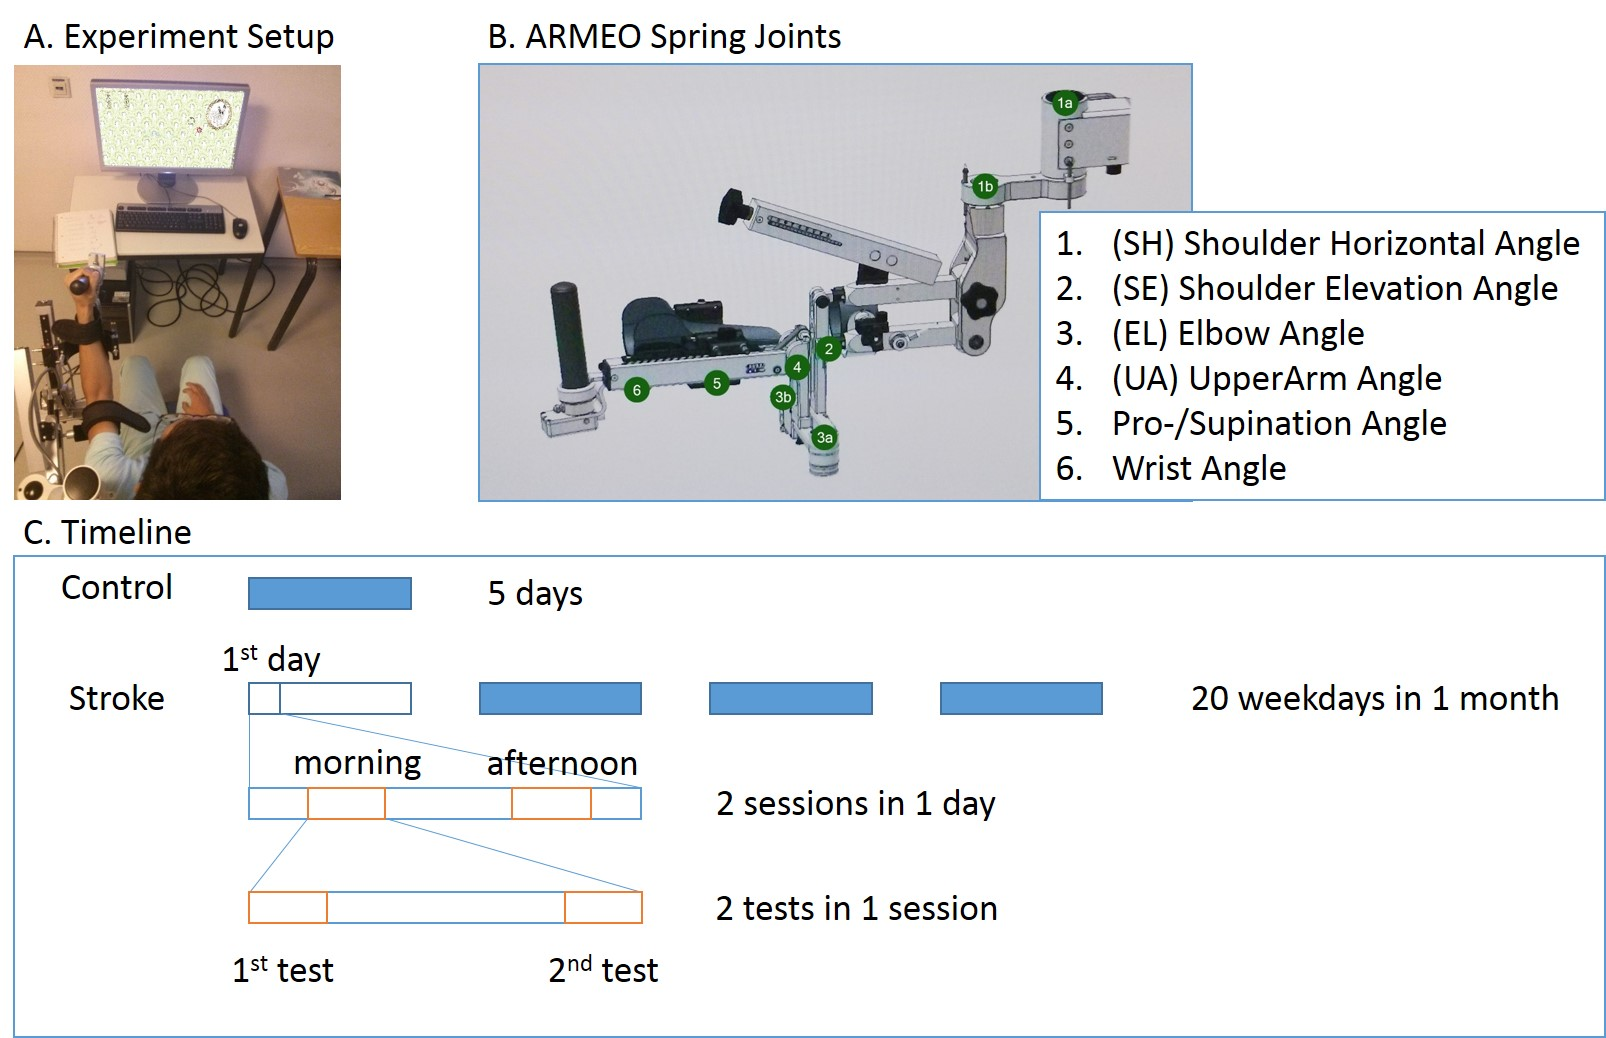
\includegraphics[width=1\linewidth]{figures/1setup&schedule}
	\caption[Experiment Setup and Schedule]
	{Experiment Setup, ARMEO Spring and Schedule. 
		A. Participants sit in front of a vertical screen on which the training games are displayed. In the ladybug test, the cursor responds to movements on a vertical plane. 
		B. Joints of ARMEO Spring. Summation of 1a and 1b is Shoulder Horizontal (SH) angle; 2 is Shoulder Elevation (SE) angle; 3a (only activated for right arm) and 3b (left arm) are elbow (EL) angles; 4 is ForeArm (FA) angle; 5 is pronation and supination angle; 6 is wrist angle.
		C. Two ladybug tests are administered at beginning and end of one session, two sessions are administered in morning and afternoon. Control group receives 5 days training, whereas stroke group receives 20 consecutive weekdays training.}
	\label{fig:1setupschedule}
\end{figure}

\begin{figure}
	\centering
	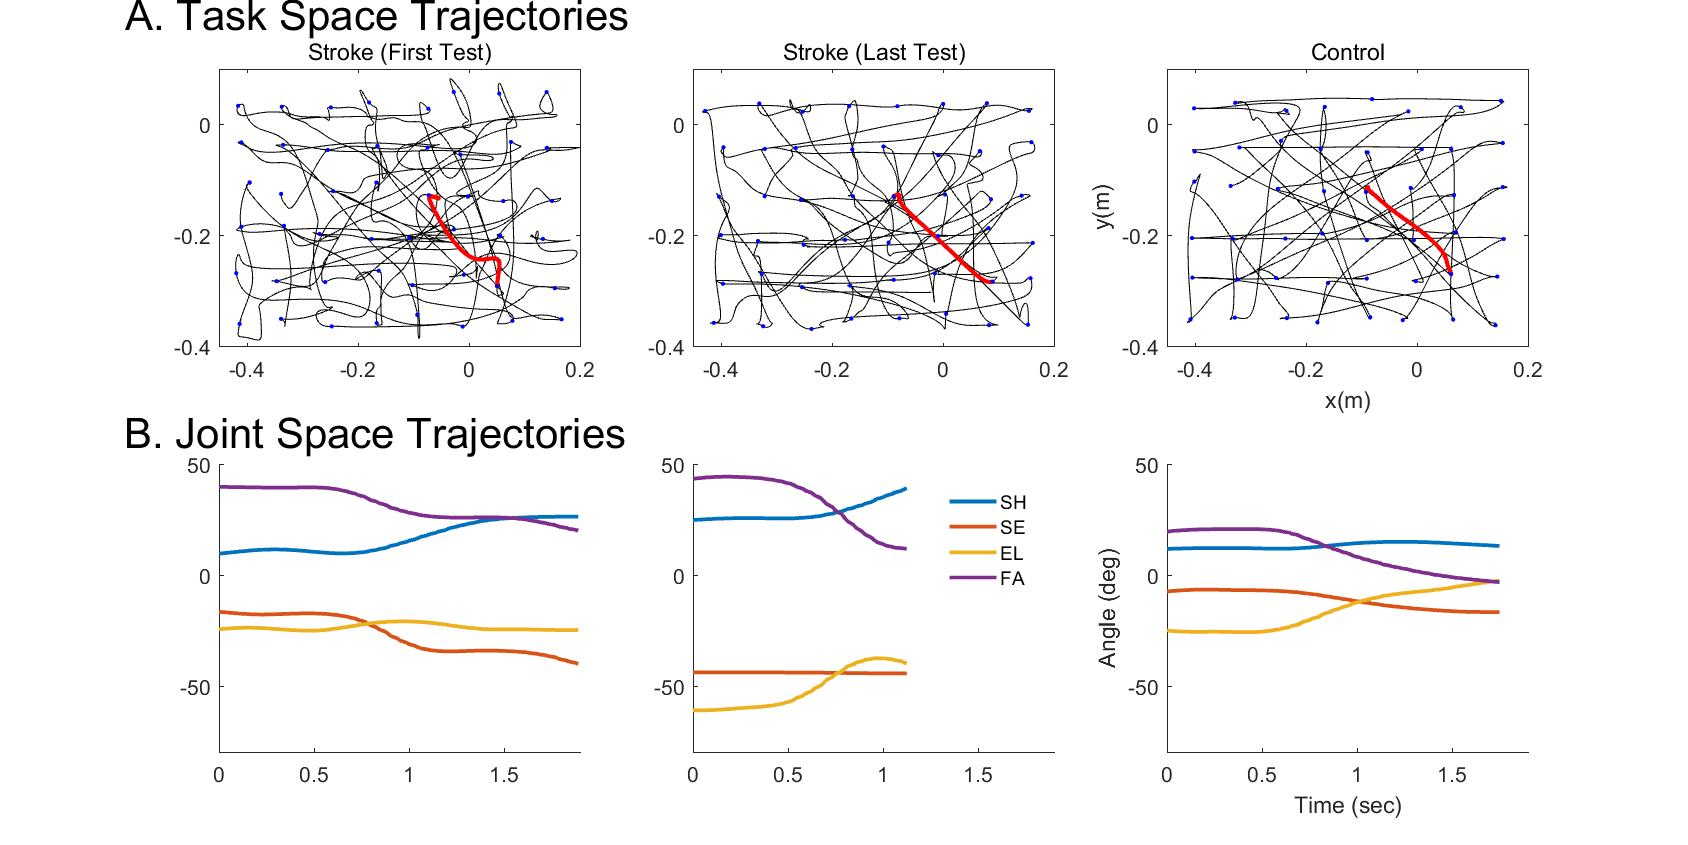
\includegraphics[width=1\linewidth]{figures/2strokeTrajExamp}
	\caption[Example trajectories]
	{Representative trajectories. 
		A. Representative task space trajectories. Trajectories after training are straighter.
		B. Representative joint space trajectories, correspond to the red part trajectories in panel A. Only the first four joints are shown.}
	\label{fig:2stroketrajexamp}
\end{figure}

\begin{figure}
	\centering
	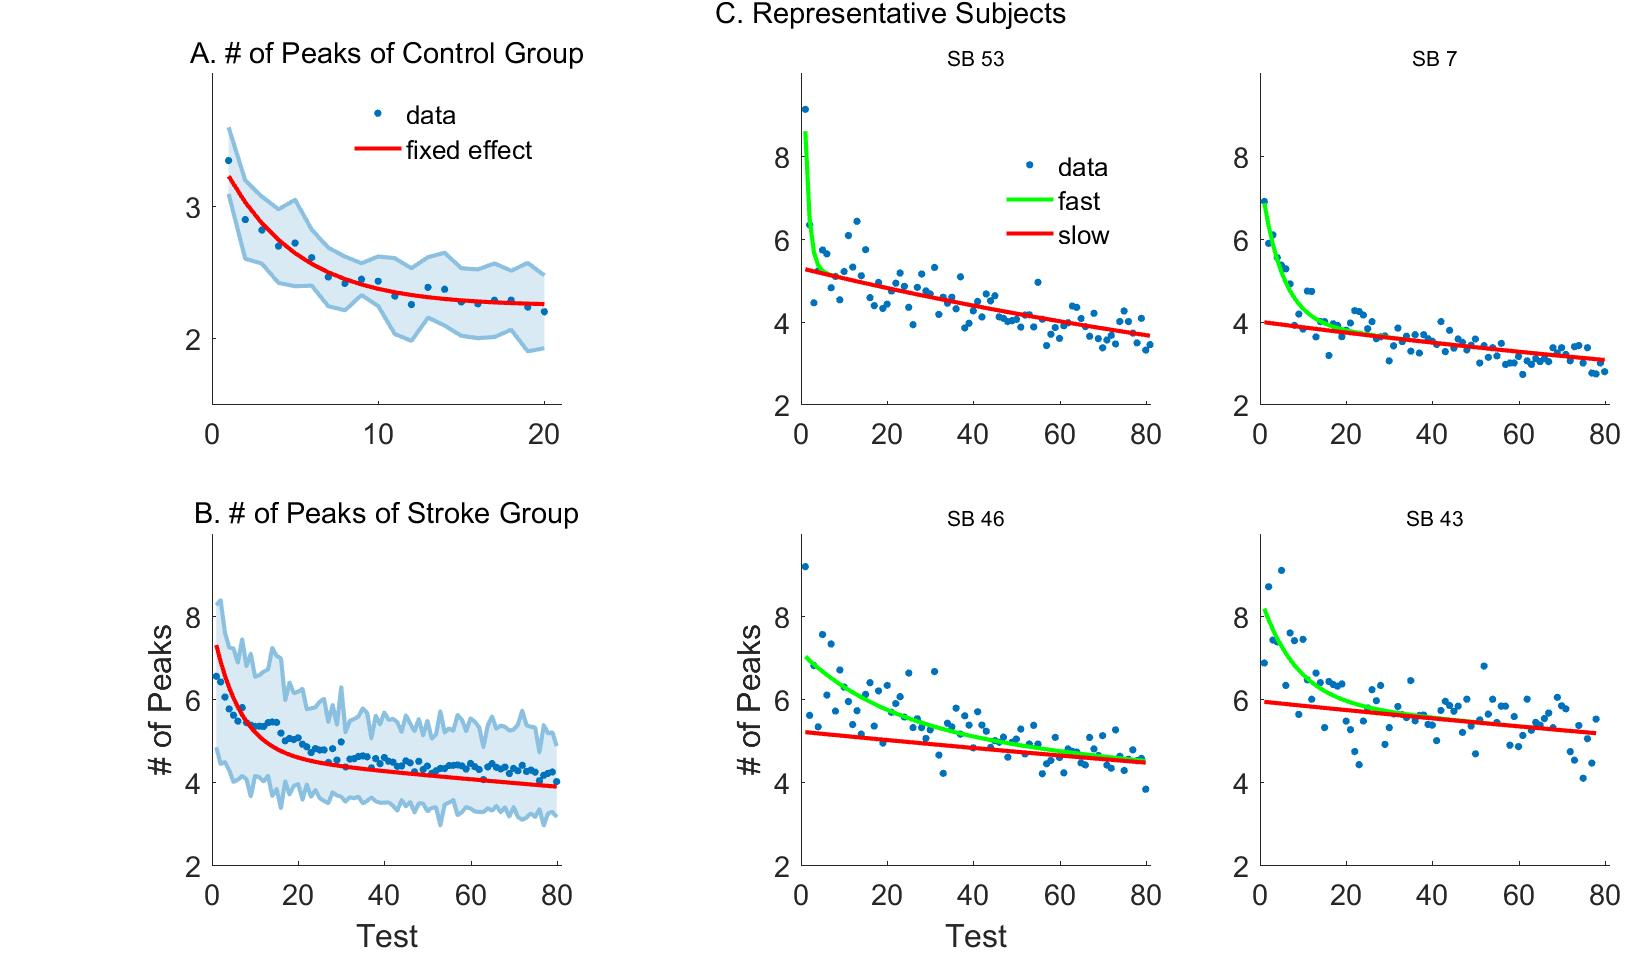
\includegraphics[width=1\linewidth]{figures/3nopFixRan}
	\caption[Double Exponential Model]
	{Double Exponential Model of Number of Peaks in Velocity Profile. 
		A,B: The fixed effect (group average) of the fitted exponential model of number of peaks. 
			Shaded area represents standard deviation;
		C: Representative participants.
			SB 53: fast learning rate and large task-irrelevant variability; 
			SB 46: slow learning rate and small task-irrelevant variability (see Fig. \ref{fig:5learnratevsnullvar} for task-irrelevant variability);
			SB 7: fast recovery rate and small initial synergy abnormality;
			SB 43: slow recovery rate and large initial synergy abnormality (see Fig. \ref{fig:6synergy} for initial synergy abnormality).
	}
	\label{fig:3nopfixran}
\end{figure}

\begin{figure}
	\centering
	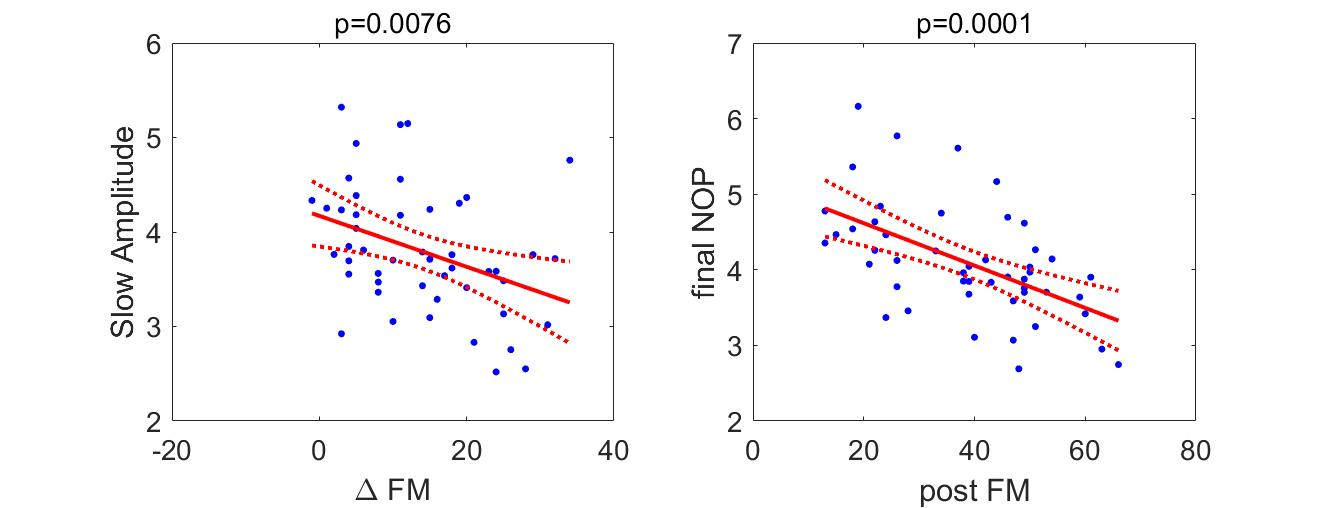
\includegraphics[width=1\linewidth]{figures/4slowComponentIsRecovery}
	\caption[Slow component corresponds to recovery as meaured by FM]
	{Slow component corresponds to recovery as measured by FM. 
		A: The number of peaks post training is correlated with FM post training;
		B: The change of number of peaks due to the slow process is correlated with the change of FM, prior and post training.
		The cyan regression line is normal least square regression; whereas the red regression line is robust regression with bisquare weight function. 
		Data points indicated by cyan crosses are outliers detected by Cook's distance.
	}
	\label{fig:4slowcomponentisrecovery}
\end{figure}

\begin{figure}
	\centering
	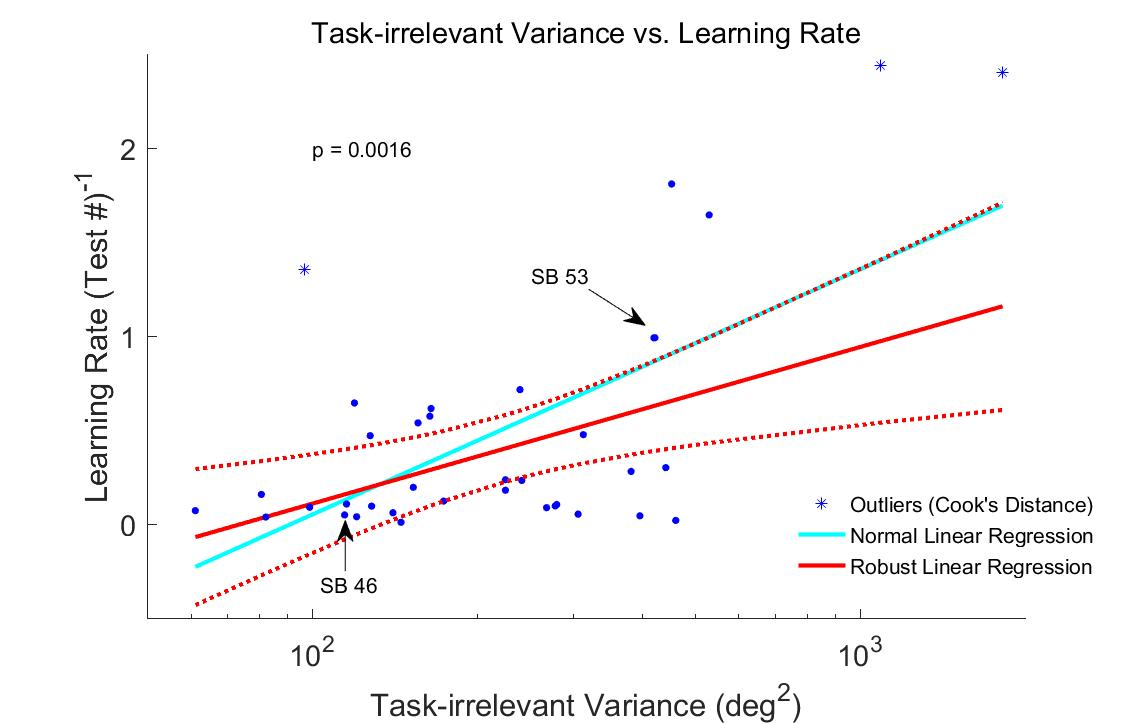
\includegraphics[width=1\linewidth]{figures/5learnRateVSnullVar}
	\caption[Exploration of Joint Redundancy facilitates learning]
	{Exploration of Joint Redundancy facilitates learning. 
		(The log of) null space variability is correlated with learning rate.
		SB 53 and 46 are representative participants, whose learning curves are shown in Fig.\ref{fig:3nopfixran}C.
		The cyan regression line is normal least square regression; whereas the red regression line is robust regression with bisquare weight function. 
		Data points indicated by cyan crosses are outliers detected by Cook's distance.}
	\label{fig:5learnratevsnullvar}
\end{figure}

\begin{figure}
	\centering
	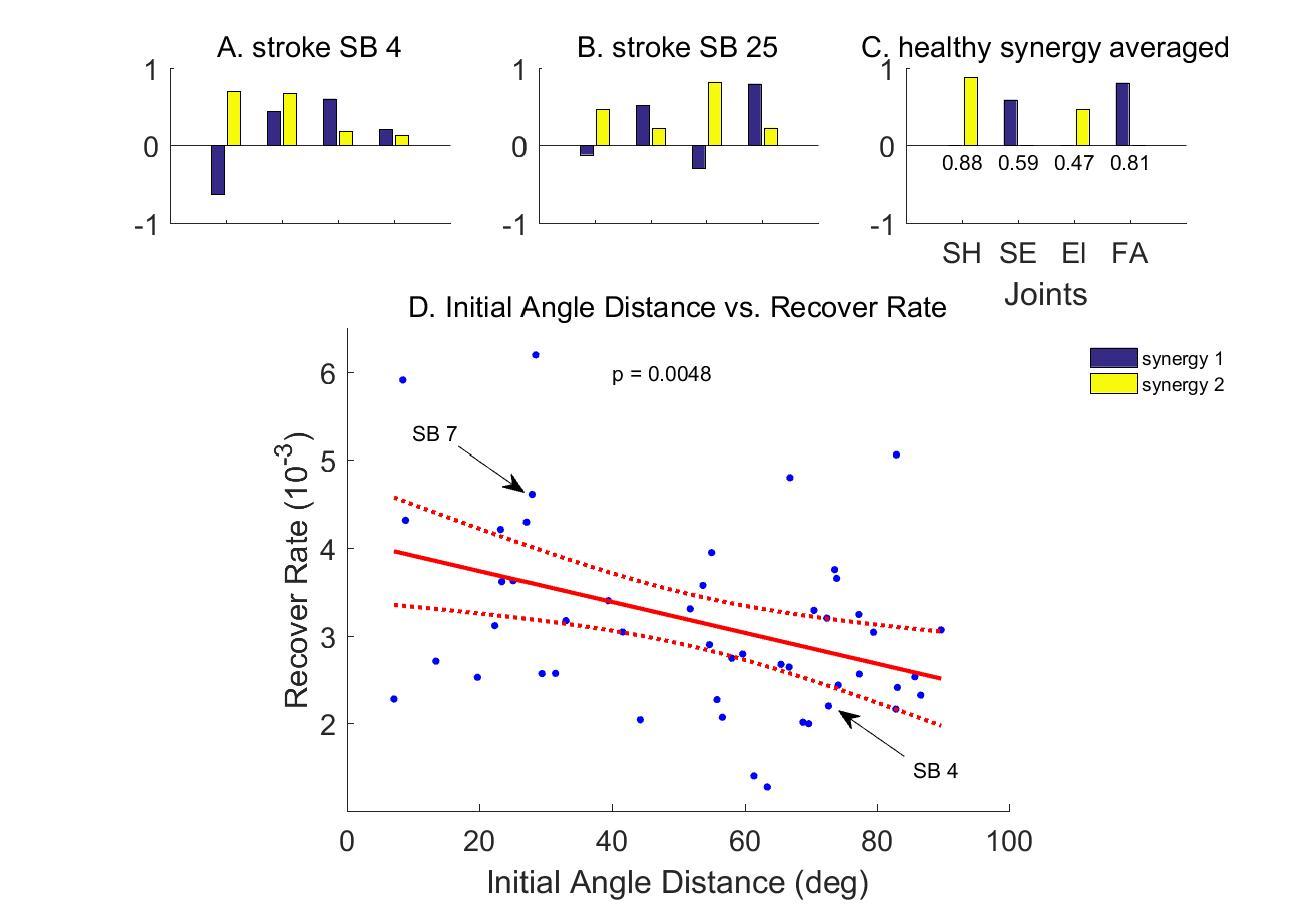
\includegraphics[width=1\linewidth]{figures/6synergy}
	\caption[Synergy Analysis]
	{Synergy Abnormality hinders recovery. 
		A-C. Radar plot of synergies. Dashed black line indicates zero. Blue and red lines are synergies.
		A. Representative participant with abnormal synergies;
		B. Representative participant with normal synergies. See Fig.\ref{fig:3nopfixran}C for their learning curves;
		C. Averaged synergies of participants in the control group;
		D. Synergy abnormality reduces recovery rate. SB 7 and 43 are representative participants, whose initial synergy patterns are shown in panel A and B, learning curves are shown in Fig.\ref{fig:3nopfixran}C.
		The cyan regression line is normal least square regression; whereas the red regression line is robust regression with bisquare weight function. 
		Data points indicated by cyan crosses are outliers detected by Cook's distance.}
	\label{fig:6synergy}
\end{figure}

